\documentclass{standalone}
\usepackage{tikz}

\newcounter{node}

\begin{document}
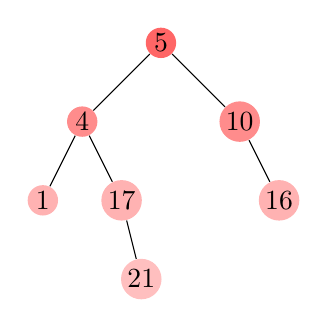
\begin{tikzpicture}
  [level distance=10mm,
    every node/.style={fill=red!60,circle,inner sep=1pt},
    level 1/.style={sibling distance=20mm,nodes={fill=red!45}},
    level 2/.style={sibling distance=10mm,nodes={fill=red!30}},
  level 3/.style={sibling distance=5mm,nodes={fill=red!25}},
]
  \node {5}
  child {node {4}
    child {node {1}}
    child {node {17}
      child[missing]
      child{node {21}}
    }
  }
  child {node {10}
    child[missing] 
    child {node {16}}
  };
\end{tikzpicture}
\end{document}





